\chapter{Energy Conservation in EPOCH Particle-in-Cell Simulations Due to Finite Numbers of Particles}
This appendix focuses on unpublished work that was done jointly with Ricky Oropeza and Joseph Smith. My contributions to this project were primarily done as a pre-candidacy student. \gls{PIC} simulations provide a useful but imperfect model of various plasma phenomena. In this work, the impact of the finite number of particles in a PIC simulation on the energy conservation is considered and explored through ultra-intense laser interactions with a thin, near solid density target in the \gls{TNSA} regime. 

\section{Background}

Explicit PIC codes tend to gain energy over time through what can be attributed as numerical errors. In this section, we consider which plasma and simulation parameters affect this numerical energy gain and derive various scalings. 

\subsection{Electric Field Fluctuations}

In PIC simulations, we compute the velocities at the next timestep through \cref{eq:v_update} which is dependent on the time-step $\Delta t$. Due to using a finite grid, approximating real particles with macro particles, and using a finite $\Delta t$, we will develop some errors in calculating the electric field $\delta E$. The corresponding force miscalculation $\delta F = q \delta E \Delta t$ would deliver an impulse $m \delta v$ and result in a velocity difference \cite{Hockney_1988_PIC} of

\begin{equation}
	\delta v = \frac{q}{m} \Delta t \delta E
\end{equation}
We can make an assumption that these field calculation errors will be randomly distributed which can be treated as a random walk in velocity space. If we consider $\Delta v$ as the total deviation of the calculated velocity from the true value, we should expect $\langle \Delta v \rangle = 0$ due to the symmetry of this random walk. However, the squared deviations on average will increase over time; for $n$ time-steps (each with the same random error $\delta E$), we would have 

\begin{equation}
	\langle \Delta v^2 \rangle = n \delta v ^2 = n \frac{q^2}{m^2} \Delta t^2 \delta E^2
\end{equation}
We can see that the average change in kinetic energy $\Delta KE \equiv \frac{1}{2} m \langle v^2 \rangle$ increases linearly with the number of time-steps $n$ \cite{Hockney_1988_PIC}. Additionally, since $\Delta KE \propto \frac{1}{m}$, the heavier particles (i.e. ions) can usually be neglected when examining the artificial heating \cite{Hockney_1988_PIC}. Hockney postulates a related expression \cite{Hockney_1971_JoCP} for $\Delta KE$ in another work as 

\begin{equation}
	\Delta KE \sim \frac{q^2}{m} \langle E^2 \rangle \tau_\text{corr} \Delta t
\end{equation}
where $\tau_\text{corr}$ can be identified with the period of plasma oscillations $\sim \omega_{p,e}^{-1}$. Then, expressing the charge of one electron macro-particle as $q = e \frac{N}{N_{mac}} = \frac{e n}{n_{mac}} = \frac{e n \Delta x^2}{n_{ppc}}$, where $\Delta x$ is the cell size\footnote{It is to the second power because we are focusing on a 2D simulation in this section.} and $n_\text{ppc}$ is the number of electron macro-particles per cell, the kinetic energy increase becomes

\begin{equation}
	\Delta KE = (\frac{e}{m_e}) \frac{e n \Delta x^2}{n_{ppc}} \langle E^2 \rangle \frac{2 \pi}{\omega_{pe}} \Delta t \label{eq:deltake}
\end{equation}
Hockney uses a result from Chapter 8.2 of Montgomery and Tidman \cite{Montgomery_1964_Plasma} for the squared electric field fluctuations

\begin{equation} 
	\frac{\langle E^2 \rangle}{8 \pi} = \frac{k_B T}{2} \int \int_{-\infty}^{+\infty} \frac{d k_x d k_y}{(2 \pi)^2} \frac{1}{(1 + (k_x^2 + k_y^2) \lambda_D^2)} 
\end{equation}
which can be solved by letting $u = k \lambda_D$ where $k = \sqrt{k_x^2 + k_y^2}$ and integrating with respect to the polar area element $k \; dk \; d \phi$

\begin{equation}
	\langle E^2 \rangle = \frac{k_B T}{4 \pi \epsilon_0 \lambda_D^2} \text{Log}(1 + u_{max^2}) \label{eq:e2}
\end{equation}
Here, $u_{max} = k_\text{max} \lambda_D$ corresponds to the maximum wavenumber $k_{max} = \frac{2 \pi}{\Delta x}$ considered which is limited by the resolution. 

\subsection{Empirical Heating Estimates}

Using Equations \ref{eq:debye}, \ref{eq:omegape}, \ref{eq:deltake}, and \ref{eq:e2} $\Delta KE$ can now be expressed as 

\begin{equation}
	\Delta KE = \frac{n_e^{3/2} \Delta x^2}{n_{ppc}} \text{Log}(1 + u_{max}^2) \label{eq:logarber}
\end{equation}
An empirical estimate for the heating can be obtained by asserting a general scaling of the heating time $\tau_H \simeq \frac{n_\text{ppc}^\alpha}{\omega_{p,e}} \left(\frac{\lambda_{D,0}}{\Delta x}\right)^d$, where $d$ (should be the dimension) and $\alpha$ are constants that can be fit through simulations. If we assert a linear energy increase with time $\frac{dT}{dt} = T_0 / \tau_H$, we develop a formula (again using Equations \ref{eq:debye} and \ref{eq:omegape}) for the linear energy increase 

\begin{equation}
	\frac{dT_{eV}}{dt_{ps}} = C_H \frac{T_{0,eV}^{1 - d/2} \Delta x_{nm}^d n_{23}^{(d + 1)/2}}{n_\text{ppc}^\alpha} \label{eq:generalizedarber}
\end{equation}
and when $\alpha = 1$ and $d = 2$, we obtain eq. (30) from Arber et al. \cite{Arber_2015_PPCF}

\begin{equation}
	\frac{dT_{eV}}{dt_{ps}} = C_H \frac{\Delta x_{nm}^2 n_{23}^{3/2}}{n_\text{ppc}} \label{eq:arber}
\end{equation}
where $C_H$ is a constant determined by the shape function and the use of current smoothing. This looks notably similar to \autoref{eq:logarber} without the log term which helps motivate its physical origin. The cell size, number density, time, and temperature are expressed in nm, $10^{23} \text{cm}^{-3}$, ps, and eV due to being convenient units for PIC simulations. A more sophisticated empirical model could also account for two dimensionless timescales: $\omega_{p, e} \Delta t$ and $v_\text{th} \Delta t$, but Hockney \cite{Hockney_1971_JoCP} notes that these can be ignored by constraining $\omega_{p,e} \Delta t$ to be $\omega_{p,e} \Delta t = \text{min}((2 \lambda_D / \Delta x)^{-1}, 1)$ \cite{Hockney_1971_JoCP}.

\section{Simulation}
\subsection{Methods}
A number of simulations were performed using the EPOCH code with a 2D(3v) geometry. The laser and target was based on the experimental facility at \gls{WP-ELL} described in \autoref{ch:6} and the relevant simulation parameters are listed in \autoref{tab:sim_params}. The laser emerges perpendicularly from one of the boundaries and is incident on a diagonally oriented target with incidence angle $45^\circ$. The target was initialized with all ions singly ionized ($\mathrm{C}^{+}$,~$\mathrm{O}^{+}$,~$\mathrm{H}^{+}$) with abundances in proportion to the chemical composition of ethylene glycol. The simulations ran for 500 fs and the energy acquired in protons, electrons, carbon, and oxygen was tracked throughout this time. This energy is highlighted in \autoref{fig:sim_energy_stack} for a simulation with many particles per cell that has a minimal amount of numerical heating.

\begin{table}
	\centering
	\begin{tabular}{c|c|c}
		\hline
		\hline
		Laser & Wavelength: Peak Intensity & 780 nm: 2.1671e18 W $\text{cm}^{-2}$\\
		\text{} & Pulse Duration: Spot Size & $\text{42}$ $\text{fs FWHM}$: $1.87$  $\mu\text{m FWHM}$\\
		\hline
		Target & Material & Ionized Ethylene Glycol\\
		\text{} & Density & $2\times10^{22}$ $\text{cm}^{-3}$\\
		\text{} & Thickness & $460$ $\text{nm}$ \\
		\hline
		Sim & Resolution & 10 nm\\
		\text{} & Total Time & 500fs\\
		\text{} & Initial Particle Temperature & 1 eV\\
		\text{} & Simulation Area & $\SI{28}{\micro \meter} \times \SI{28}{\micro \meter}$ \\
		\hline
		\hline
	\end{tabular}
	\caption{Summary of Simulation Parameters (constant)}
	\label{tab:sim_params}
\end{table}

\begin{figure}
	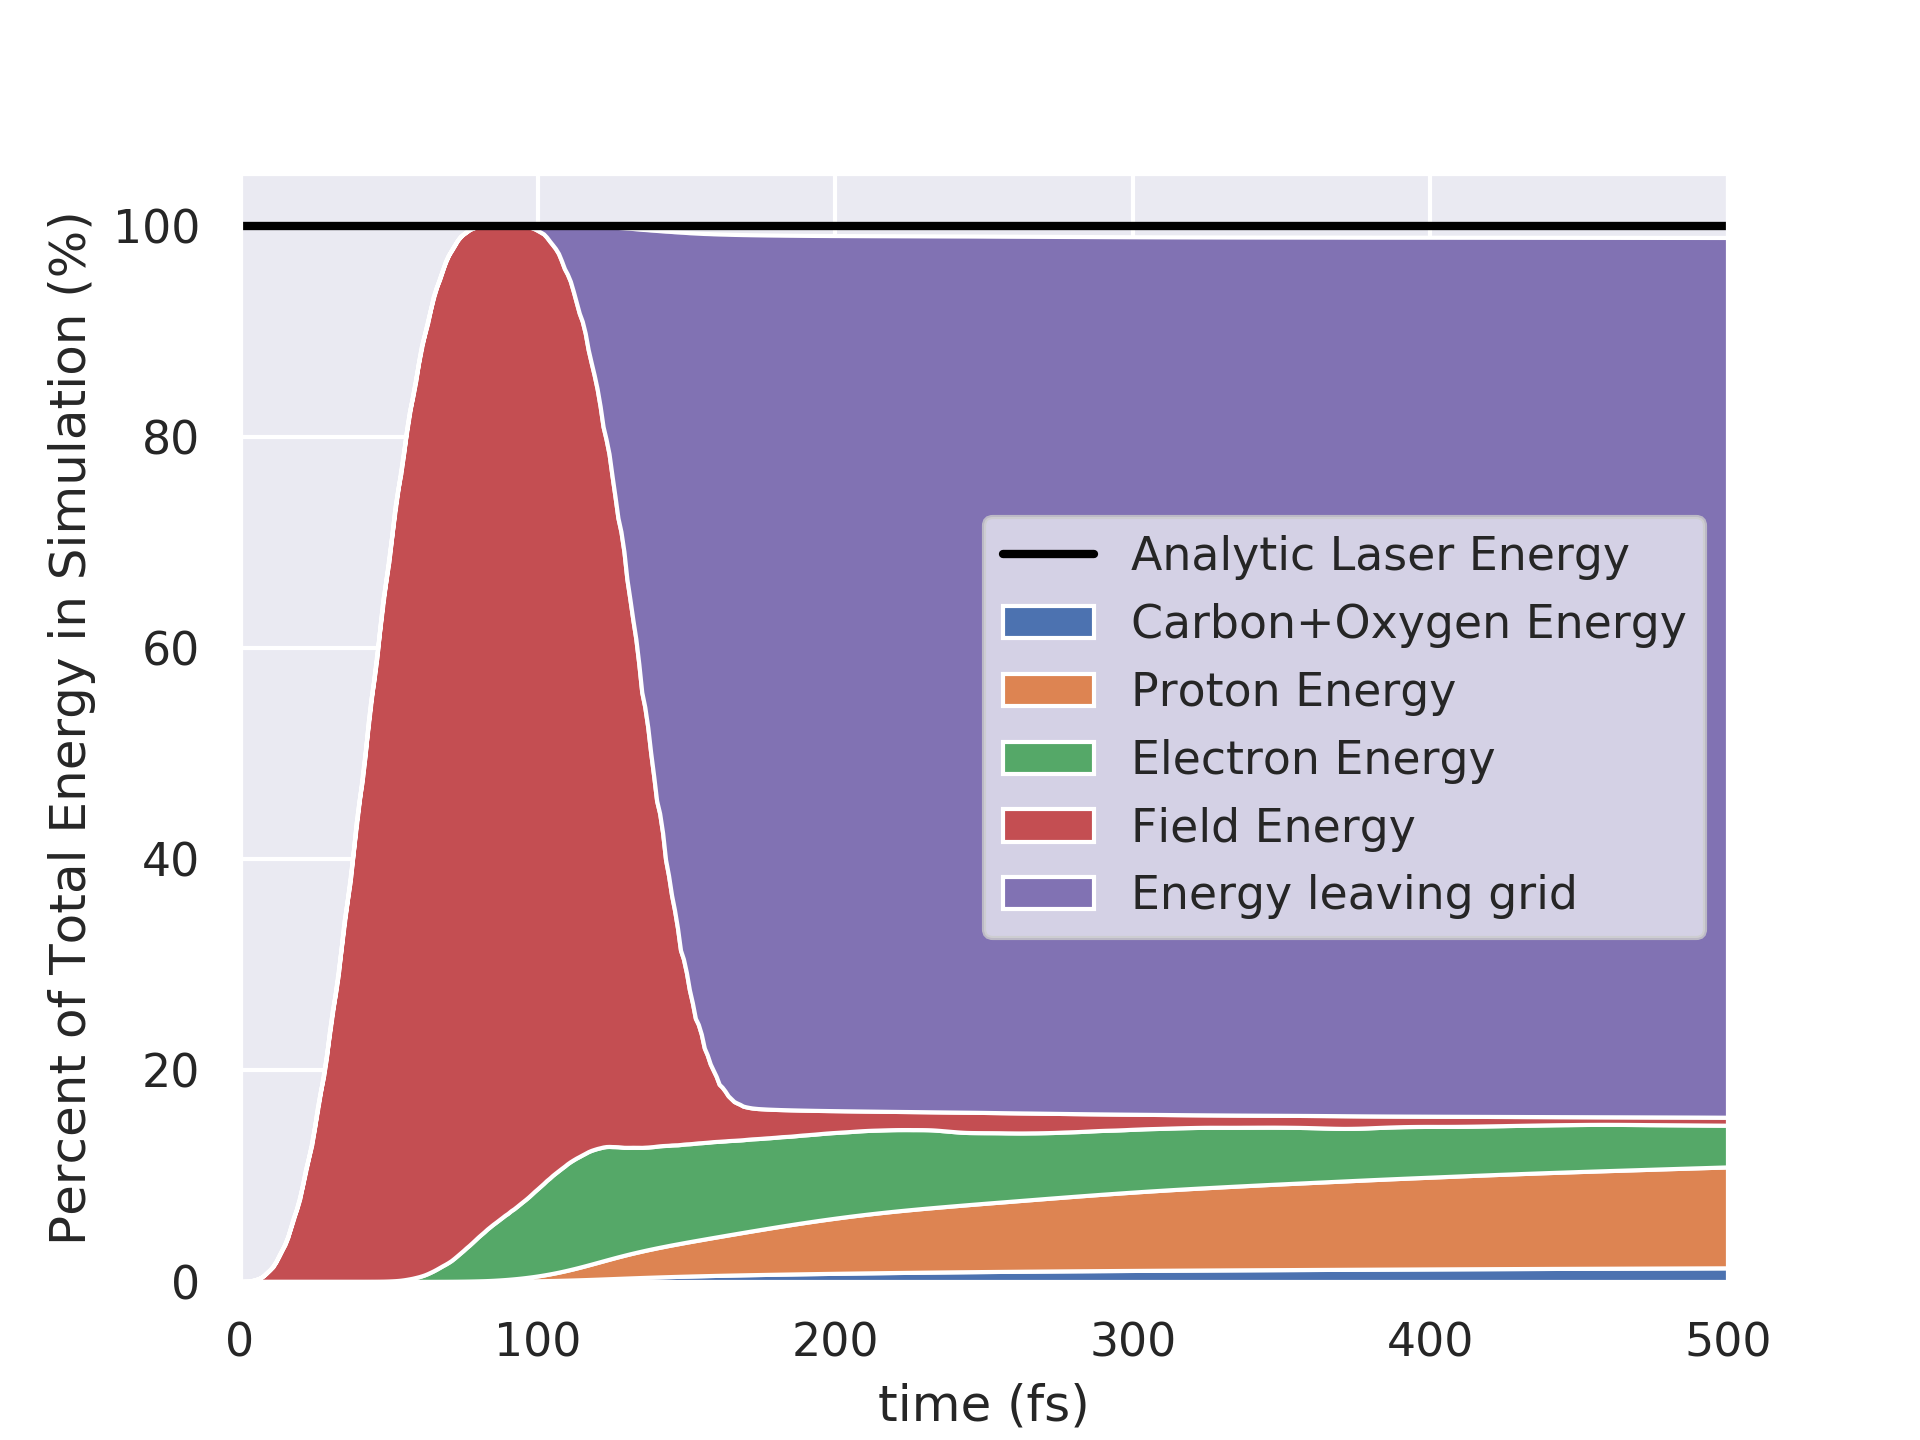
\includegraphics[width=0.9\linewidth]{planning/images/arber/Energy_Plot_2D.png}
	\caption{The total energy and how it is distributed over time in the simulation. The black line is amount of energy that should be in the system from the laser pulse in the simulation.} \label{fig:sim_energy_stack} 
\end{figure}

\subsection{Results}
According to \autoref{eq:arber}, if the number of particles per cell is low, one should expect more numerical heating and the energy in electrons (the green region in \autoref{fig:sim_energy_stack}) to be larger than expected. However, in this simulation setup, there are multiple species which can all have different numbers of particles per cell. From running these simulations, it became clear that the electron particles per cell is not the only relevant number (even though it is the most influential). When oxygen and carbon ionize, they release electrons, so the carbon and oxygen particles per cell should also be important quantities that arise in a scaling like \autoref{eq:arber}. To analyze the effect of varying the number of particles per cell, we conducted a set of 44 simulations that are listed in \autoref{tab:all_ppc_sims}. The specific numbers of particles per cell were chosen by utilizing a Sobol sequence which attempts to fill up the 4D parameter space (particles per cell for each species) in such a way to not leave large gaps (CITATION). This table clearly shows how changing the number of particles per cell (in an otherwise identical simulation setup) influences the amount of energy that gets delivered to each species. The true conversion efficiencies should be close to the values for the simulations with many particles per cell (e.g. simulations 42 and 43) and conversion efficiencies higher than these simulations should be regarded as numerical effects.

\renewcommand{\arraystretch}{1}
\setlength{\tabcolsep}{0.25em}
\begin{table}
	\centering
	\begin{tabular}{c|c|c|c|c|c|c|c|c|c}
		\hline
		Sim \# & $n_\text{ppc,e}$ & $n_\text{ppc,p}$ & $n_\text{ppc,O}$ & $n_\text{ppc,C}$ & $n_\text{ppc,total}$ &$\eta_e$ at~120fs & $\eta_p$ at~500fs  & $\eta_O$ at~500fs & $\eta_C$ at~500fs\\
		\hline
		1 & 5.0 & 38.0 & 42.0 & 59.0 & 144.0 & 11.435 & 9.672 & 0.816 & 0.671\\
		2 & 7.0 & 121.0 & 60.0 & 100.0 & 288.0 & 11.260 & 9.748 & 0.817 & 0.643\\
		\textbf{3} & 9.0 & 9.0 & 9.0 & 9.0 & 36.0 & \textbf{11.977} & \textbf{6.917} & \textbf{1.158} & \textbf{0.887}\\
		\textbf{4} & 9.0 & 9.0 & 9.0 & 9.0 & 36.0 & \textbf{11.907} & \textbf{6.881} & \textbf{1.137} & \textbf{0.868}\\
		5 & 15.0 & 94.0 & 173.0 & 100.0 & 382.0 & 11.198 & 9.552 & 0.811 & 0.642\\
		6 & 18.0 & 52.0 & 145.0 & 200.0 & 415.0 & 11.114 & 9.567 & 0.781 & 0.631\\
		7 & 20.0 & 66.0 & 118.0 & 45.0 & 249.0 & 11.190 & 9.171 & 0.808 & 0.660\\
		8 & 23.0 & 23.0 & 164.0 & 255.0 & 465.0 & 11.032 & 9.368 & 0.781 & 0.641\\
		9 & 26.0 & 37.0 & 282.0 & 136.0 & 481.0 & 11.051 & 9.368 & 0.758 & 0.633\\
		10 & 29.0 & 86.0 & 36.0 & 164.0 & 315.0 & 11.107 & 9.119 & 0.786 & 0.669\\
		\textbf{11} & 29.0 & 86.0 & 36.0 & 36.0 & 187.0 & \textbf{11.134} & \textbf{8.695} & \textbf{0.826} & \textbf{0.685}\\
		\textbf{12} & 29.0 & 86.0 & 36.0 & 36.0 & 187.0 & \textbf{11.113} & \textbf{8.635} & \textbf{0.807} & \textbf{0.685}\\
		13 & 32.0 & 77.0 & 227.0 & 227.0 & 563.0 & 10.953 & 9.300 & 0.759 & 0.634\\
		\textbf{14} & 35.0 & 35.0 & 54.0 & 54.0 & 178.0 & \textbf{11.065} & \textbf{8.915} & \textbf{0.791} &  \textbf{0.678}\\
		\textbf{15} & 35.0 & 35.0 & 54.0 & 54.0 & 178.0 & \textbf{11.045} & \textbf{8.916}& \textbf{0.783} & \textbf{0.664}\\
		16 & 37.0 & 26.0 & 100.0 & 173.0 & 336.0 & 11.046 & 9.329 & 0.749 & 0.646\\
		17 & 40.0 & 74.0 & 218.0 & 127.0 & 459.0 & 10.984 & 9.308 & 0.758 & 0.637\\
		18 & 43.0 & 43.0 & 191.0 & 264.0 & 541.0 & 10.978 & 9.432 & 0.730 & 0.627\\
		19 & 46.0 & 91.0 & 91.0 & 36.0 & 264.0 & 11.030 & 8.938 & 0.768 & 0.667\\
		20 & 49.0 & 60.0 & 64.0 & 209.0 & 382.0 & 10.980 & 9.335 & 0.727 & 0.636\\
		21 & 52.0 & 18.0 & 255.0 & 91.0 & 416.0 & 10.990 & 9.298 & 0.748 & 0.658\\
		22 & 54.0 & 54.0 & 154.0 & 154.0 & 416.0 & 10.947 & 9.352 & 0.727 &  0.630\\
		23 & 57.0 & 12.0 & 127.0 & 145.0 & 341.0 & 11.106 & 9.465 & 0.732 & 0.651\\
		\textbf{24} & 60.0 & 49.0 & 27.0 & 27.0 & 163.0 & \textbf{11.111} & \textbf{8.655} & \textbf{0.782} & \textbf{0.691}\\
		\textbf{25} & 60.0 & 49.0 & 27.0 & 27.0 & 163.0 & \textbf{11.102} & \textbf{8.661} & \textbf{0.783} & \textbf{0.679}\\
		26 & 60.0 & 49.0 & 27.0 & 245.0 & 381.0 & 11.071 & 9.330 & 0.712 & 0.652\\
		27 & 63.0 & 97.0 & 291.0 & 54.0 & 505.0 & 10.954 & 9.281 & 0.744 & 0.637\\
		28 & 66.0 & 20.0 & 264.0 & 191.0 & 541.0 & 11.018 & 9.543 & 0.738 & 0.650\\
		\textbf{29} & 69.0 & 69.0 & 18.0 & 18.0 & 174.0 & \textbf{11.117} & \textbf{8.319} & \textbf{0.819} & \textbf{0.705}\\
		\textbf{30} & 69.0 & 69.0 & 18.0 & 18.0 & 174.0 & \textbf{11.108} & \textbf{8.339} & \textbf{0.809} & \textbf{0.717}\\
		31 & 74.0 & 40.0 & 182.0 & 18.0 & 314.0 & 11.043 & 8.949 & 0.774 & 0.649\\
		32 & 77.0 & 32.0 & 82.0 & 82.0 & 273.0 & 10.965 & 9.376 & 0.734 & 0.653\\
		33 & 83.0 & 72.0 & 245.0 & 27.0 & 427.0 & 10.960 & 9.160 & 0.739 & 0.641\\
		34 & 86.0 & 29.0 & 73.0 & 273.0 & 461.0 & 10.999 & 9.560 & 0.704 & 0.634\\
		35 & 89.0 & 89.0 & 45.0 & 118.0 & 341.0 & 10.893 & 9.352 & 0.701 & 0.643\\
		36 & 91.0 & 46.0 & 236.0 & 182.0 & 555.0 & 10.887 & 9.563 & 0.698 & 0.622\\
		37 & 94.0 & 15.0 & 209.0 & 64.0 & 382.0 & 10.948 & 9.401 & 0.724 & 0.648\\
		38 & 97.0 & 63.0 & 109.0 & 236.0 & 505.0 & 10.895 & 9.587 & 0.703 & 0.626\\
		39 & 119.0 & 119.0 & 70.0 & 70.0 & 378.0 & 10.885 & 9.397 & 0.712 & 0.644\\
		40 & 131.0 & 82.0 & 131.0 & 131.0 & 475.0 & 10.800 & 9.557 & 0.689 & 0.614\\
		41 & 187.0 & 203.0 & 11.0 & 13.0 & 414.0 & 11.061 & 8.580 & 0.783 & 0.725\\
		\textbf{42} & 257.0 & 64.0 & 92.0 & 58.0 & 471.0 & \textbf{10.852} & \textbf{9.663} & \textbf{0.694} & \textbf{0.619}\\
		\textbf{43} & 257.0 & 64.0 & 92.0 & 58.0 & 471.0 & \textbf{10.834} & \textbf{9.611} & \textbf{0.687} & \textbf{0.624}\\
		44 & 294.0 & 164.0 & 32.0 & 41.0 & 531.0 & 10.915 & 9.484 & 0.713 & 0.652\\ \hline
	\end{tabular}
	\caption{Particles per cell and conversion efficiencies for all 44 simulations.}
	\label{tab:all_ppc_sims}
\end{table}
To analyze which factors influence the numerical heating gain, we first looked at a spearman correlation matrix in \autoref{fig:correlation} which can show the correlations between the relevant simulation inputs and outputs in \autoref{tab:all_ppc_sims}. When looking at the row with the electron conversion efficiency -- which is the quantity most relevant to artificial heating -- we see that the electron particles per cell has the strongest correlation. However, the correlations with oxygen and carbon particles per cell are not negligible either. As mentioned earlier, the non-zero correlations should be influenced by the electrons that get ionized from carbon and oxygen throughout the simulations. From this physical insight, I came up with a formula to modify the electron particles per cell to the effective particles per cell

\begin{figure}
	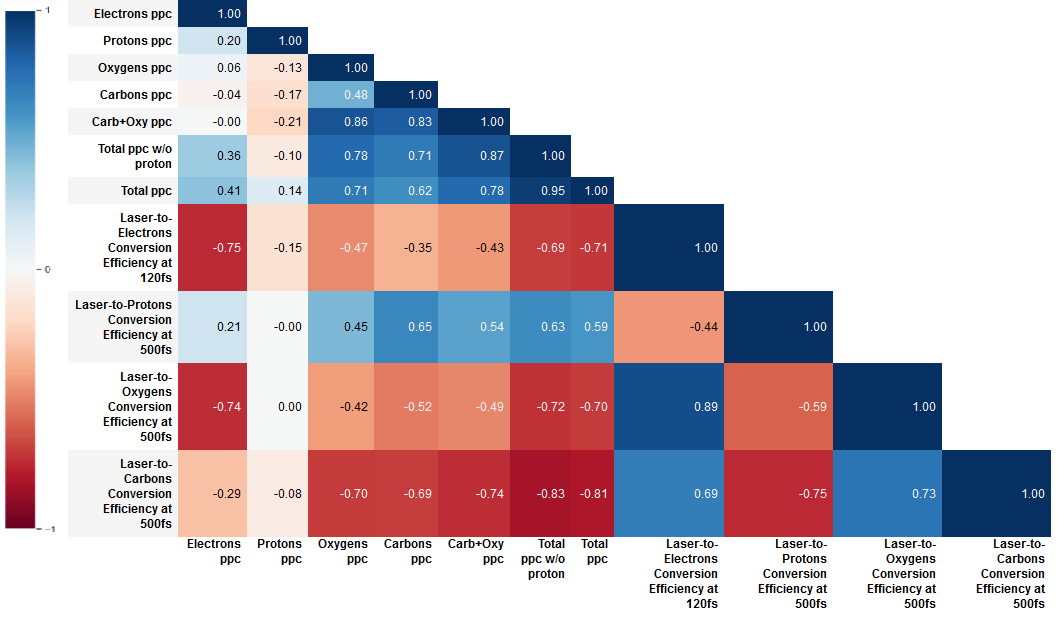
\includegraphics[width=0.9\linewidth]{planning/images/arber/corr_matrix.png}
	\caption{A spearman correlation matrix of the inputs and outputs of all the simulations} \label{fig:correlation}
\end{figure}


\begin{equation}
	\frac{1}{n_\mathrm{ppc,eff}} \rightarrow \frac{1}{n_\mathrm{ppc,e}} + \frac{Z^*_O-1}{n_\mathrm{ ppc,O}} +\frac{Z^*_C-1}{n_\mathrm{ppc,C}}
	\label{eq:neff}
\end{equation}
where $Z_O^*$ and $Z_C^*$ are the effective ionization states\footnote{The ionization states were subtracted by 1 because the simulation started out singly ionized.} of oxygen and carbon that were extracted from the simulations and reported in \autoref{tab:Zeff}. These ionization states were calculated by taking a sum of the ionization state (e.g. $Z = {1, 2, 3, \ldots}$) weighted by the macro-particle count in each state and dividing by the total macro-particle count.

\begin{table}
	\centering
	\begin{tabular}{c|c|c}
		\hline
		Sim \# & $Z_O^*$ & $Z_C^*$ \\ \hline
		1 & 2.176142756 & 2.375174888 \\ 
		2 & 2.327658955 & 2.421891557 \\ 
		3 & 3.143308831 & 2.915937614 \\ 
		4 & 3.154803787 & 2.927684972 \\ 
		5 & 2.496638636 & 2.527135231 \\ 
		6 & 2.441216019 & 2.508804562 \\ 
		7 & 2.584687195 & 2.627203273 \\ 
		8 & 2.387585622 & 2.486757853 \\ 
		9 & 2.392126498 & 2.531181839 \\ 
		10 & 2.564046446 & 2.634346386 \\ 
		11 & 2.543839748 & 2.644390761 \\ 
		12 & 2.412445491 & 2.530124101 \\ 
		13 & 2.291655813 & 2.471869382 \\ 
		14 & 2.421709685 & 2.575093874 \\ 
		15 & 2.406534033 & 2.577752667 \\ 
		16 & 2.264716398 & 2.48188157 \\ 
		17 & 2.246043951 & 2.485791191 \\ 
		18 & 2.178764825 & 2.432073341 \\ 
		19 & 2.361060481 & 2.5738224 \\ 
		20 & 2.167570944 & 2.425260178 \\ 
		21 & 2.185477012 & 2.443200305 \\ 
		22 & 2.140609639 & 2.414440722 \\ 
		23 & 2.126992307 & 2.407471987 \\ 
		24 & 2.142192439 & 2.403501354 \\ 
		25 & 2.393986109 & 2.625379573 \\ 
		26 & 2.412863167 & 2.619551359 \\ 
		27 & 2.17524236 & 2.480400199 \\ 
		28 & 2.046239782 & 2.345317225 \\ 
		29 & 2.518141858 & 2.688972667 \\ 
		30 & 2.514367481 & 2.694657044 \\
		31 & 2.372678171 & 2.648680619 \\ 
		32 & 2.071785068 & 2.380991226 \\ 
		33 & 2.208017982 & 2.547074535 \\ 
		34 & 1.992876487 & 2.30745977 \\ 
		35 & 2.046732563 & 2.365068347 \\ 
		36 & 1.952194826 & 2.286210998 \\ 
		37 & 2.035659427 & 2.37849725 \\ 
		38 & 1.930691366 & 2.266609743 \\ 
		39 & 1.987261106 & 2.345904477 \\ 
		40 & 1.897934111 & 2.254506282 \\ 
		41 & 2.494837238 & 2.719446774 \\ 
		42 & 1.878585202 & 2.274410676 \\ 
		43 & 1.870289532 & 2.27367933 \\ 
		44 & 1.961455166 & 2.362095052 \\ \hline
	\end{tabular}
	\caption{Effective ion charge for all simulations}
	\label{tab:Zeff}
\end{table}

\begin{figure}
	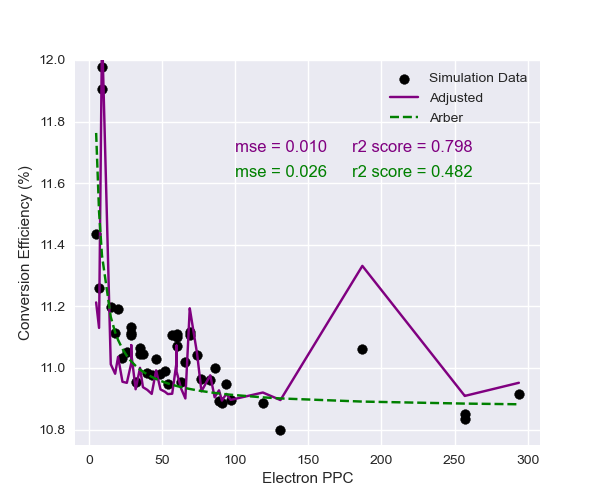
\includegraphics[width=0.9\linewidth]{planning/images/arber/L-E_1param_eppc.png}
	\caption{Plot of Arber et al. model (\autoref{eq:arber}) compared to the effective particle per cell model (using \autoref{eq:neff}) plotted against the electron particles per cell.} \label{fig:ppc_model}
\end{figure}
 In \autoref{fig:ppc_model}, the original Arber scaling from \autoref{eq:arber} and adjusted scaling (with \autoref{eq:neff}) are plotted as a green dashed line and purple solid line with a scatter plot of the simulation data. While the Arber model is a smooth function of the electron particles per cell, the data clearly has points where it jumps up and down which the adjusted model captures more of. It is important to note that both models only used one free parameter: the heating constant $C_H$ from \autoref{eq:arber}. The plot itself shows the $r^2$ correlation score and \gls{MSE} which is more favorable for the model adjusted to effective particles per cell. 

\section{Conclusion}
Throughout this chapter, I explored a common question that many simulation researchers face: how many particles per cell should be utilized per species in a \gls{PIC} simulation? I first addressed this question theoretically by building upon the work of Hockney and Eastwood \cite{Hockney_1988_PIC} and Arber et al. \cite{Arber_2015_PPCF}. Then, I utilized a set of 2D \gls{PIC} simulations\footnote{These were conducted by Ricky Oropeza.} to evaluate the effectiveness of the Arber et al. model (\autoref{eq:arber}) with and without the effective particle per cell adjustment (\autoref{eq:neff}) in capturing the data. While the Arber et al. model definitely has correct trends with the electron particles per cell, it does not fully capture information about the other species. The effective particle per cell is a better predictor of the numerical heating, but not perfect by any means. 

To continue this work, I believe an extensive set of thousands of \gls{PIC} simulations would need to be conducted over a more exhaustive combination of particles per cell. These simulations should also be performed over several different resolutions (i.e. $\lambda_D / \Delta x$) due to making a noticeable difference in the scaling properties of the numerical heating from my own experience. Current simulation practitioners rely on an archaic method of deciding the numbers of particles per cell: starting out at a low resolution and increasing resolution and particles per cell until the simulation results stay relatively consistent. With modern day advances in computing clusters and machine learning capabilities, I believe that more useful empirical estimates can be developed to both understand the nature of numerical heating better and save time for computational scientists.
